\begin{itemize}
	\item Short PiC (EMSES) explanation
	\item Experimental set up
	\item 
\end{itemize}
\subsection{Numerical methods}

To solve the problem numerically we use the EMSES code. EMSES uses the standard PIC method for plasma simulations.
In the code we are able to define a spacecraft body, and the code then calculates the potential on that body using the capacitance matrix method.
Although EMSES has the capability to do a full electromagnetic calculation, we have opted to use the poisson's equation 
solver for electrostatic problems. In the EMSES system we can define sunlit surfaces based upon an angle, and a current 
desity. Sunlit surfaces will then emmit electrons based upon a energy distribution. For a complete description of EMSES' capabilities
see \citep{nakashima_ohhelp:_2009} Parameters are choosen to simulate the sun at the earth, but with an enhanced flux to emphasize the effect in question. 

\subsection{Theoretical calculations}

\begin{equation}
\begin{split}
 I_i = &
    \left\{\begin{array}{ccc}
       A|q|n_\infty\sqrt{\frac{8 k T_i}{\pi m_i}} (without flow)\\
       \frac{1}{6}A |q|n_\infty V + \frac{5}{6} A |q| n_\infty \sqrt{\frac{8 k T_i}{\pi M_i}}(with flow)
      \end{array}\right. \\
  I_e = & -A|q|n_\infty \sqrt{\frac{8 k T_e}{\pi m_e}}exp\Big(\frac{|q|\Phi_d}{k T_e}\Big)\\
  I_{ph} = & \frac{1}{6} AJ_s
\end{split}
\label{thin sheet potential} 
\end{equation}

\begin{equation}
\begin{split}
 \Phi_d = & \frac{k T_e}{|q|}ln\Big(\sqrt{\frac{T_i}{T_e}}\sqrt{\frac{m_e}{m_i}}+\frac{J_s}{6 n_\infty |q|}\sqrt{\frac{\pi m_e}{8 k T_e}}\Big) + \Phi_0 \\
 \Phi_d = & \frac{k T_e}{|q|}ln\Big(\frac{5}{6}\sqrt{\frac{T_i}{T_e}}\sqrt{\frac{m_e}{m_i}}+\frac{V}{6}\sqrt{\frac{\pi m_e}{8 k T_e}} + \frac{J_s}{6 n_\infty |q|}\sqrt{\frac{\pi m_e}{8 k T_e}} \Big) \\
 \Phi_0 = & k T_{ph}, \ V = speed\ of\ flow
\end{split}
\label{thin sheet potential 2} 
\end{equation}



\subsection{Test case setup}

We wish to simulate the effects of Photon emmited electrons in different test cases, and have thus set up the following
6 cases:
\begin{center}
    \begin{tabular}{ | l | l | l | p{5cm} |}
    \hline
    Case & Plasme flow & Photon emission  \\ \hline
     1: & 41600 $\vec{e_x}$ m/s  & 0 \\ \hline
     2: & -41600 $\vec{e_z}$ m/s & 0 \\ \hline
     3: & -41600 $\vec{e_y}$ m/s & 0 \\ \hline
     4: & 41600 $\vec{e_x}$ m/s & $-10^{-3} A/m^{3}$ $\vec{e_x}$\\ \hline
     5: & -41600 $\vec{e_z}$ m/s & $-10^{-3} A/m^{3}$ $\vec{e_x}$\\ \hline
     6: & -41600 $\vec{e_y}$ m/s & $-10^{-3} A/m^{3}$  $\vec{e_x}$\\
    \hline
    \end{tabular}
\end{center}

So test case 1-4, 2-5, and 3-6 are the ``same'' cases exept that we run the simulation with and without
photon emission to compare the cases two and two. 

\begin{figure}
        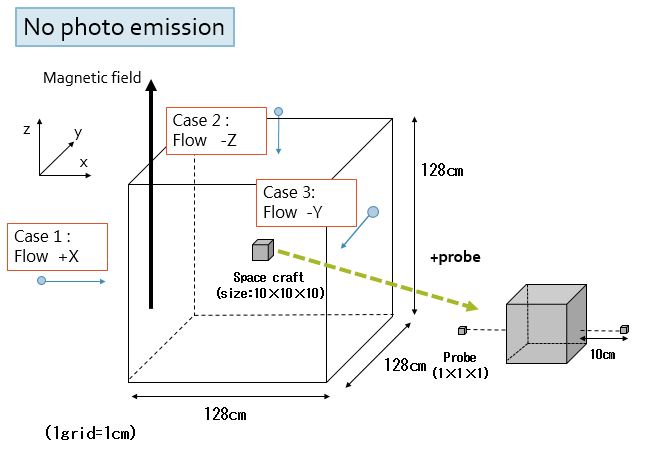
\includegraphics[width = 0.5 \textwidth]{images/picture_simulation1.png}
        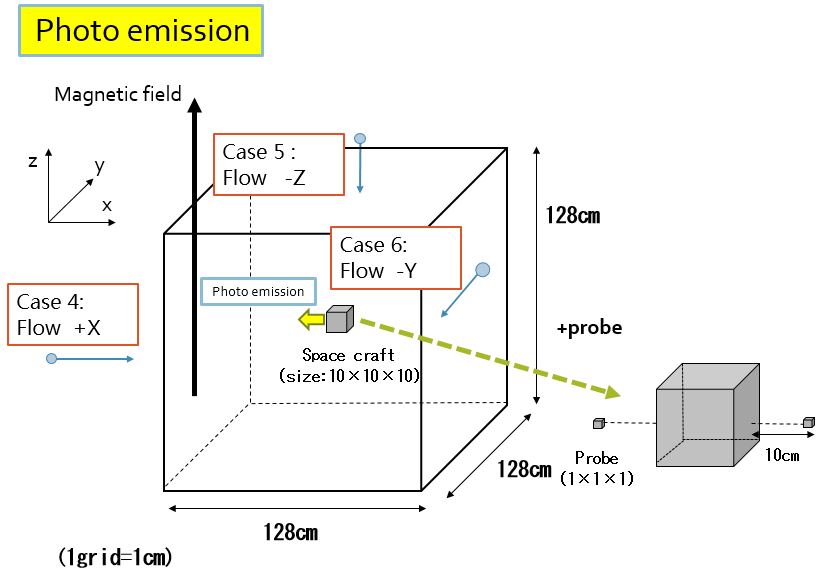
\includegraphics[width = 0.5 \textwidth]{images/picture_simulation2-2.png}
        \caption{Reseach about spacecraft and surroundings without P-E and without.Left figure is no P-E simulation cases.Right figure is P-E simulation cases.}
    \end{figure}  
